%!TEX root = report.tex
\chapter{Étude Comportementale}

\section{Introduction du Chapitre}
%TODO

\section{Navigation dans l'interface utilisateur}

\begin{figure}
\center
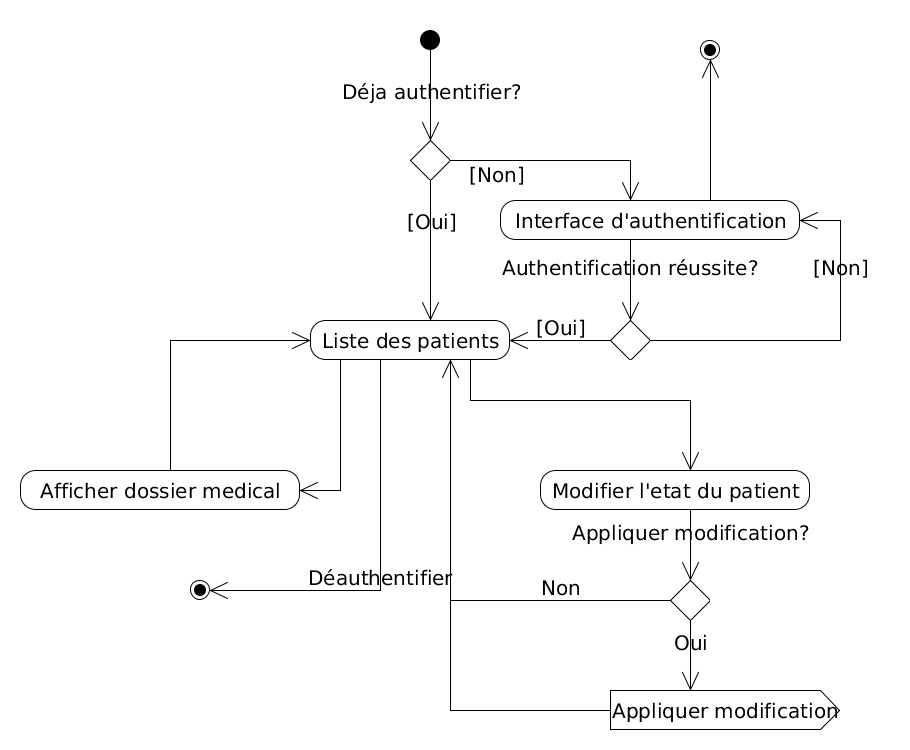
\includegraphics[width=0.8\textwidth]{diagrams/user_navigation}
\caption{Diagramme \gls{uml} d'activités de la navigation dans l'interface utilisateur.}
\label{fig:uml_act_ui}
\end{figure}

La figure \ref{fig:uml_act_ui} modélise par un diagramme \gls{uml} d'états le schéma que l'utilisateur suit pour naviguer dans l'interface utilisateur de notre application. Quelque Capture d'écran sont inclue pour illustrer le processus (figures \ref{fig:sc_login}, \ref{fig:sc_urgent}, \ref{fig:sc_display}, \ref{fig:sc_options}).

\begin{figure}
\center
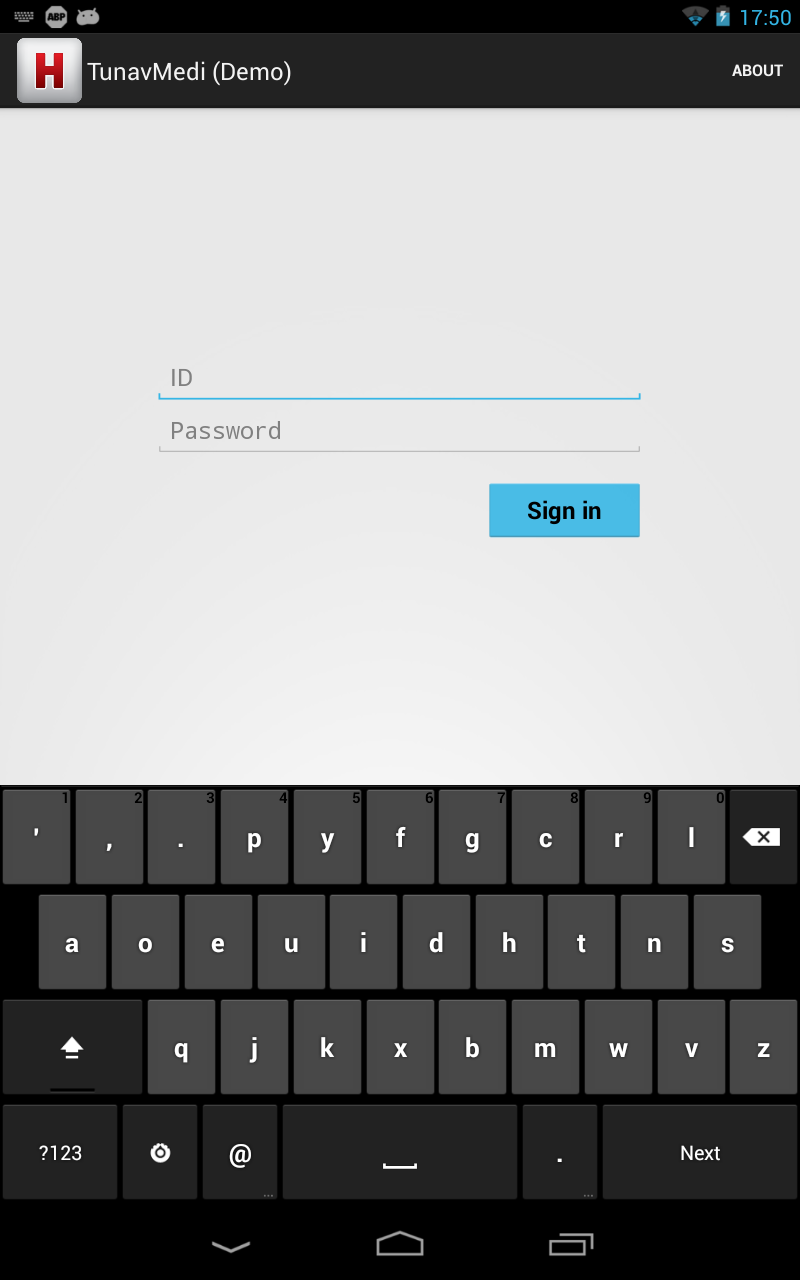
\includegraphics[height=0.4\textheight]{sc_login}
\caption{Interface graphique d'authentification.}
\label{fig:sc_login}
\end{figure}

\begin{figure}
\center
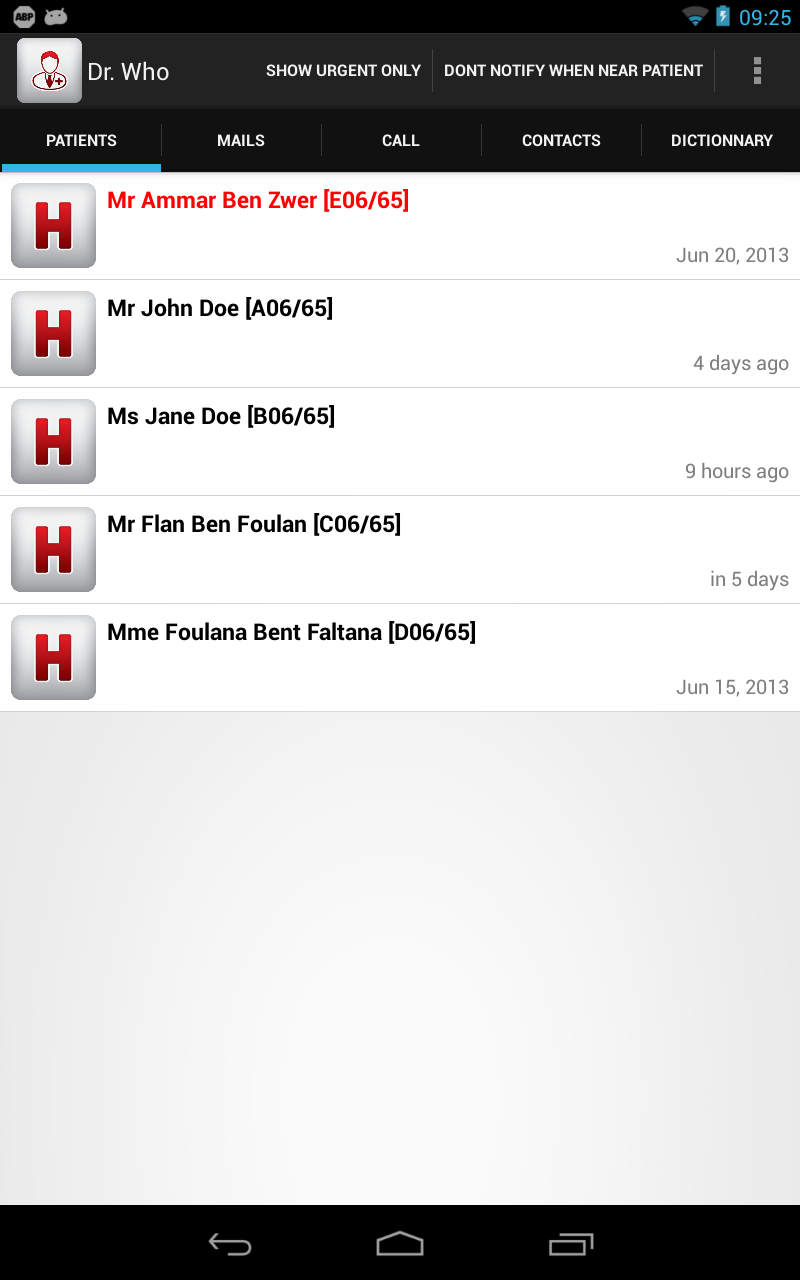
\includegraphics[height=0.4\textheight]{sc_urgent}
\caption{Capture écran de l'interface utilisateur de la liste des patients}
\label{fig:sc_urgent}
\end{figure}

\begin{figure}
\center
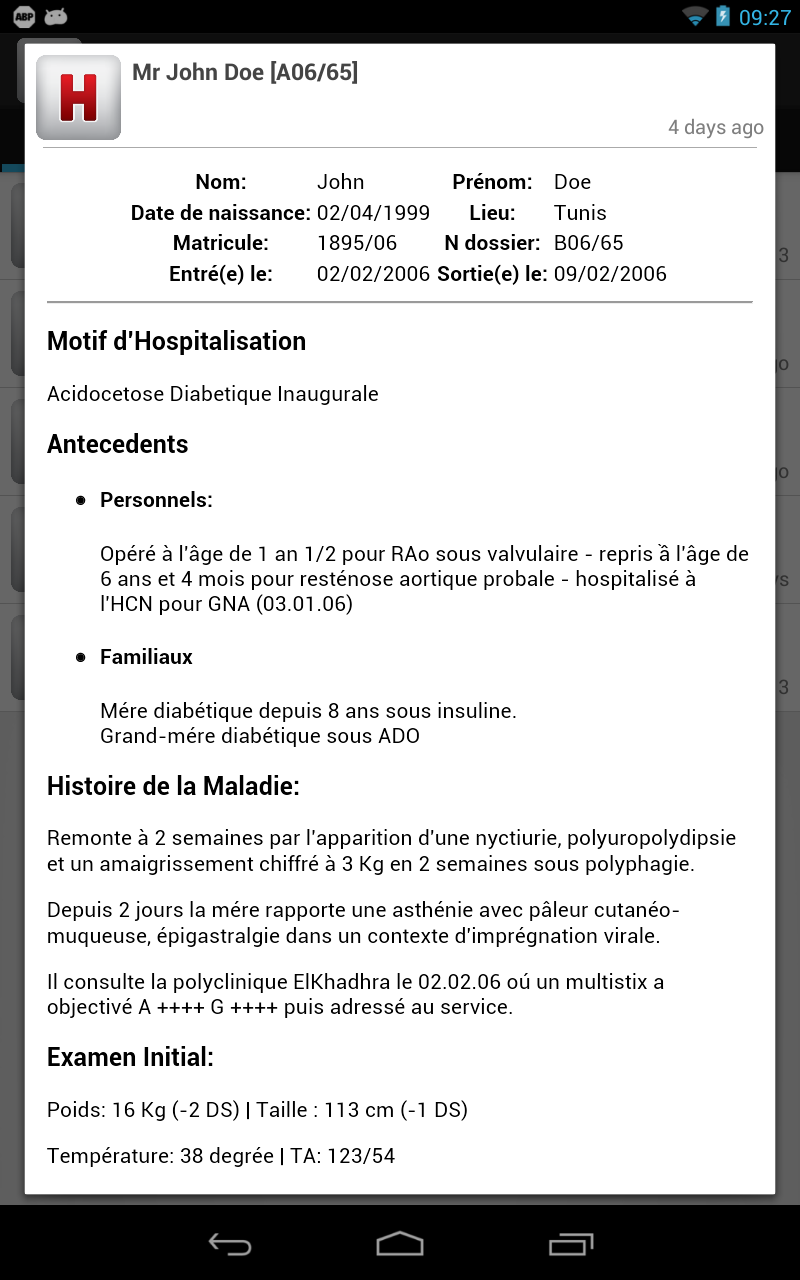
\includegraphics[height=0.4\textheight]{sc_display}
\caption{Capture écran de l'interface utilisateur relative à l'affichage du dossier médical du patient.}
\label{fig:sc_display}
\end{figure}

\begin{figure}
\center
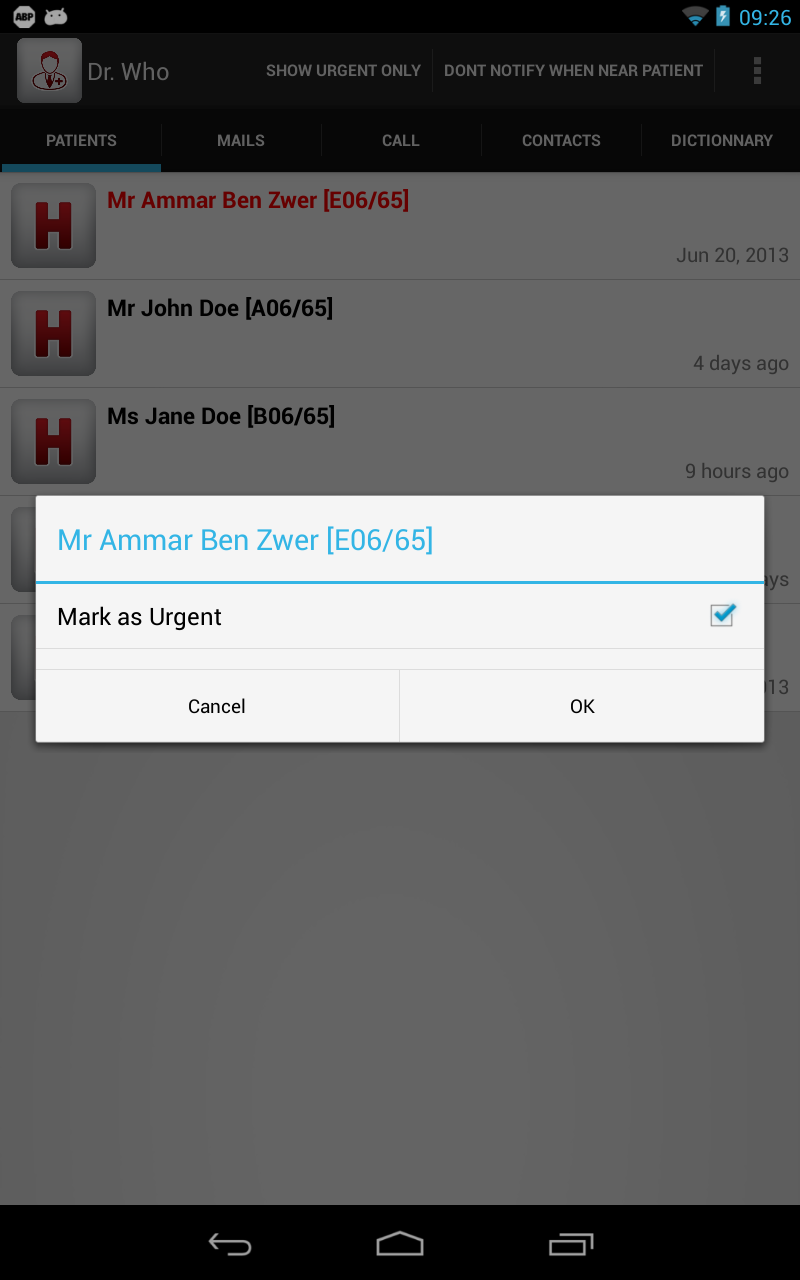
\includegraphics[height=0.4\textheight]{sc_options}
\caption{Capture écran de l'interface utilisateur affichée l'or de la modification de l’état du patient}
\label{fig:sc_options}
\end{figure}

\section{Authentification}

\begin{figure}
\center
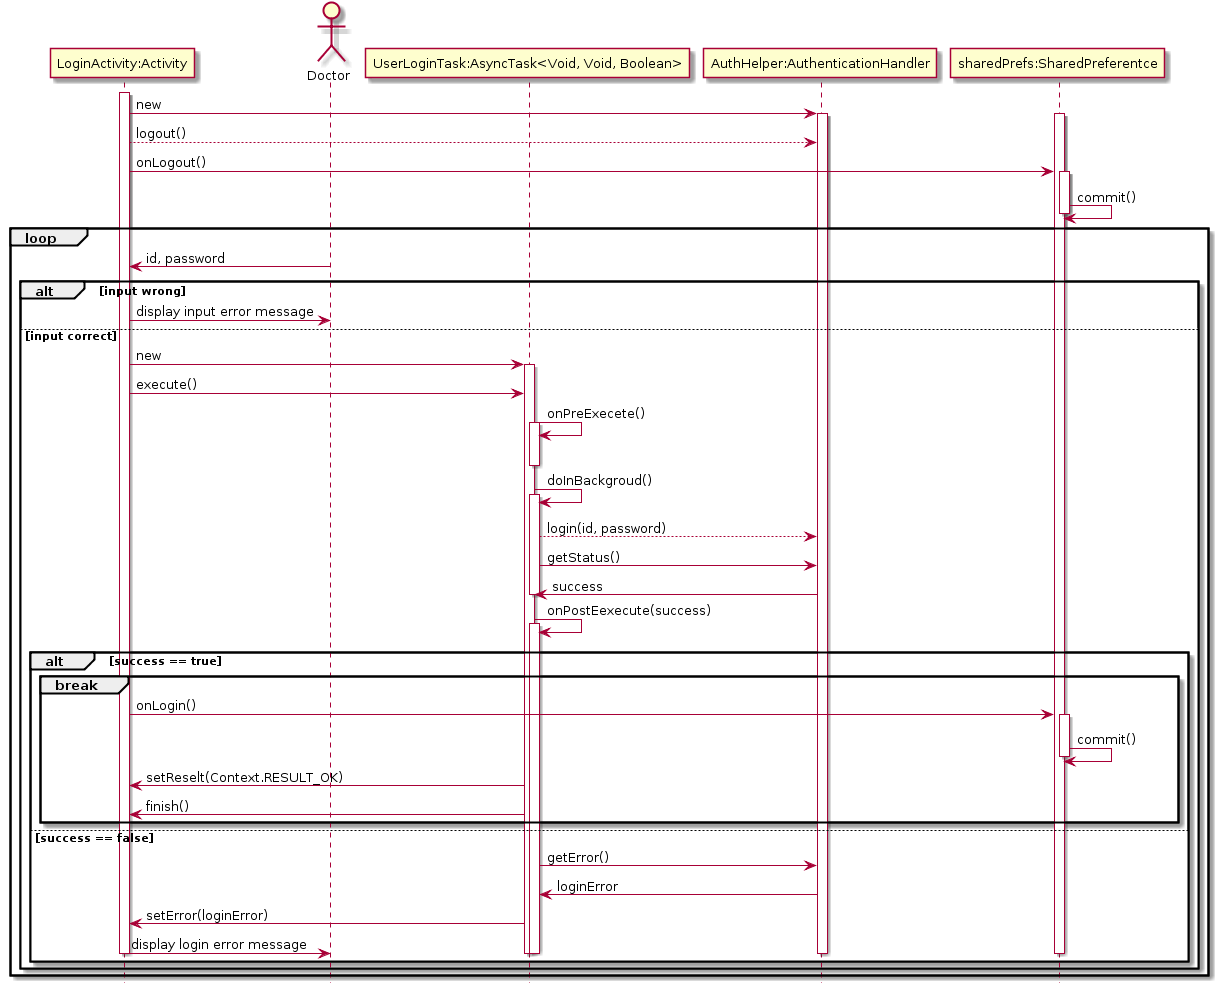
\includegraphics[angle=-90, width=\textwidth]{diagrams/seq_auth}
\caption{Diagramme \gls{uml} de séquence d'authentification.}
\label{fig:seq_auth}
\end{figure}

La figure \ref{fig:seq_auth} présente le comportement de l'application pour réaliser l'opération d'authentification de l'utilisateur à travers un diagramme de séquence \gls{uml}. On peut décrire textuellement le processus par les points suivants:

\begin{description}

\item[Acteurs:] Docteur.

\item[Pré-condition:] Le docteur est déjà inscrit dans la base de données du service et son identifiant et mot de passe lui sont fournit.

\item[Post-condition:] L'utilisateur est authentifier.

\item[Scénario nominal:]

\begin{enumerate}

\item L'utilisateur lance ou retourne à l'application mobile donc \dev{MainActivity}.

\item \dev{MainActivity} détecte que l'utilisateur n'est pas déjà authentifié et actionne l'\gls{ui} d'authentification (appel à \dev{LoginActivity}).

\item L'utilisateur saisit son identifiant et mot de passe.

\item L'application interpelle le service pour vérifier que la combinaison identifiant / mot de passe est correcte.

\item Le service distant retourne une réponse favorable, \dev{LoginActivity} enregistre les données relative à l'utilisateur.

\item \dev{LoginActivity} invoque \dev{MainActivity}.

\end{enumerate}

\item [Enchaînement alternatif:]

\begin{itemize}

\item 2.a L'utilisateur est déjà authentifier:

\begin{enumerate}

\item La séquence d'authentification est sautée.

\end{enumerate}

\item 3.a L’identifiant et / ou le mot de passe comporte des erreurs (champs vide, mot de passe comporte moins des caractères que le minimum):

\begin{enumerate}

\item Affichage d'un message d'erreur.

\end{enumerate}

\item 5.a Le service distant retourne une réponse défavorable:

\begin{enumerate}

\item Le message d'erreur est extrait de l'interface d'authentification.

\item \dev{LoginActivity} affiche le message d'erreur.

\end{enumerate}

\end{itemize}

\end{description}

\section{Afficher La Liste des Patients}
\section{Afficher Le dossier médical du patient}

\begin{figure}
\center
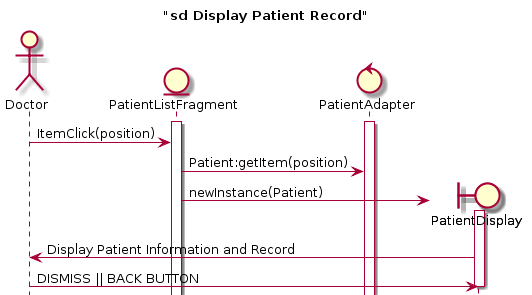
\includegraphics[width=0.8\textwidth]{diagrams/seq_display}
\caption{Diagramme de séquence \gls{uml} de l'affichage du dossier médical du patient.}
\label{fig:seq_display}
\end{figure}

La figure \ref{fig:seq_display} présente le comportement de l'application pour réaliser l'opération de l'affichage du dossier médical du patient à travers un diagramme de séquence \gls{uml}. On peut décrire textuellement le processus par les points suivants:

\begin{description}

\item[Acteurs:] Docteur.

\item[Pré-condition:] Le docteur s'est déjà authentifier et il se trouve sur l'interface de la liste des patients.

\item[Post-condition:] Le docteur à peut visualiser le dossier médical du patient qu'il à sélectionné.

\item[Scénario nominal:]

\begin{enumerate}

\item Le docteur clic sur un patient de la liste

\item \dev{PatientListFragment} détecte le clic et demande l'objet de type \dev{Patient} qui correspond au patient sélectionné par la méthode \dev{PatientAdapter.getItem()}.

\item L'objet \dev{Patient} reçu, \dev{PatientListFragment} crée une boite de  dialogue de type \dev{PatientDisplay} en lui passant l'objet Patient

\item \dev{PatientDisplay} affiche le dossier médical du patient.

\item Le docteur peut retourné à la liste des patient par un clic en dehors de la boite de dialogue ou par le bouton (retour).

\end{enumerate}

\end{description}

\section{Modification de l'Etat du patient}

\begin{figure}
\center
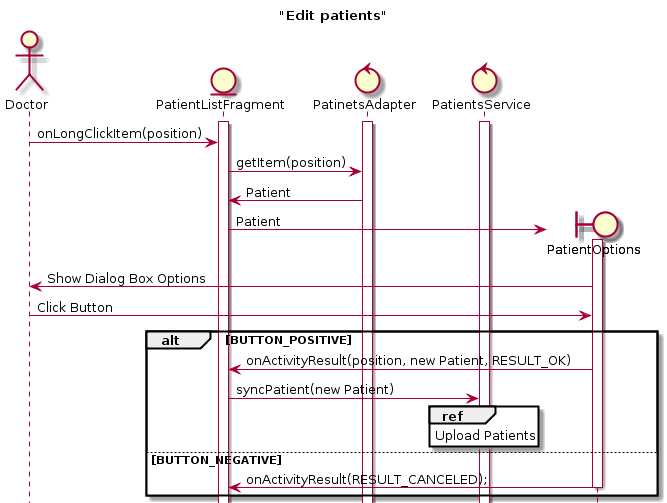
\includegraphics[width=0.8\textwidth]{diagrams/seq_editpatient}
\caption{Diagramme de séquence \gls{uml} de modification du status du patient.}
\label{fig:seq_edit}
\end{figure}

La figure \ref{fig:seq_edit} présente le comportement de l'application pour réaliser l'opération de modification du status du patient (état normal ou état critique) à travers un diagramme de séquence \gls{uml}. On peut décrire textuellement le processus par les points suivants:

\begin{description}

\item[Acteurs:] Docteur.

\item[Pré-condition:] Le docteur s'est déjà authentifier et il se trouve sur l'interface de la liste des patients.

\item[Post-condition:] Le docteur à peut modifier le status du patient qu'il a sélectionné.

\item[Scénario nominal:]

\begin{enumerate}

\item Pour modifier le status d'un patient (cet patient est un cas urgent ou non) le médecin localise le patient dans la liste est fait un clic long sur son entrée.

\item Le \dev{PatientListFragment} détecte le clic long sur l'entrée du patient et demande au \dev{PatientAdapter} un objet patient à partir de sa position dans la liste à travers la méthode \dev{getItem()}.

\item L'objet \dev{Patient} correspondant au patient sélectionner reçu, le \dev{PatientListFragment} crée une boite de dialogue de type \dev{PatientOptions}.

\item La boite de dialogue \dev{PatientOptions} présente à l'utilisateur un checkbox avec deux boutons: bouton (OK) et bouton (Cancel) (figure \ref{fig:sc_options}).

\item Le médecin effectue le changement selon ses souhait et clic sur le bouton (OK).\label{item:alt}

\item \dev{PatientOptions} retourne à la \dev{PatientListFragment} l'objet Patient
mis à jour ainsi que sa position dans la liste et un drapeau
(RESULT\_OK).

\item La \dev{PatientListFragment} fait appel au \dev{PatientService} à travers sa méthode \dev{syncPatient()} et lui passe le patient modifier.

\item Le \dev{PatientService} effectue la séquence de mise à jour des patients (voir \ref{s:patientUpdate}).

\end{enumerate}

\item [Enchaînement alternatif:]

\begin{itemize}

\item \ref{item:alt}.a Le docteur clic sur le bouton (Cancel) au lieu du bouton (OK).
\begin{enumerate}

\item \dev{PatientOptions} retourne à la \dev{PatientListFragment} avec le drapeau (RESULT\_CANCELED).

\end{enumerate}

\end{itemize}


\end{description}

\section{Mise à jour des patients à partir du terminal}
\label{s:patientUpdate}

\begin{figure}
\center
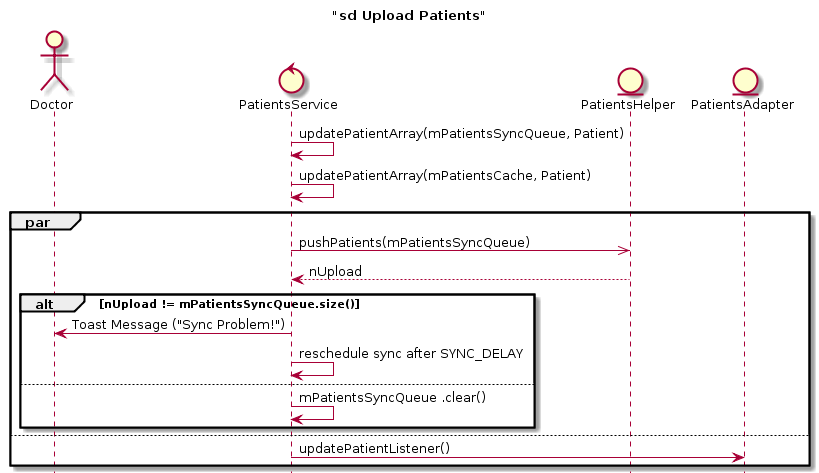
\includegraphics[width=0.9\textwidth]{diagrams/seq_uploadpatients}
\caption{Diagramme de séquence \gls{uml} Mise à jour des patients.}
\label{fig:seq_uploadpatients}
\end{figure}

La figure \ref{fig:seq_uploadpatients} présente le comportement de l'application pour réaliser l'opération de mise à jour d'un patient à travers un diagramme de séquence \gls{uml}. On peut décrire textuellement le processus par les points suivants:


\begin{description}

\item[Acteurs:] Docteur.

\item[Pré-conditions:] Le patient mis à jour par le docteur est disponible au \dev{PatientsService}, Le terminal est connecter au service distant.

\item[Post-conditions:] Le patient mis à jour par le docteur est transférer vers le service distant ou en cas de problème sauvegarder pour une mis à jour ultérieur.

\end{description}

\paragraph{Scénarios nominal:}

\begin{enumerate}

\item Le \dev{PatientsService} procède à la mise à jour de deux \dev{ArrayList}: \dev{mPatientSyncQueue} qui sert pour le fils d'attente pour les mises à jour et \dev{mPatientCache} que contient la liste des patients utilisé par notre application.

\item Deux démarches sont exécutées en parallèle:\label{enu:par}

\begin{enumerate}[label=\ref{enu:par}.\Alph*]

\item Premier démarche.\label{enu:par1}

\begin{enumerate}[label=\ref{enu:par1}.\arabic*]

\item \dev{PatientService} fait appel au \dev{PatientHelper} pour le transfer, en retour il reçoi le nombre des patients mis à jour.

\item Le nombre des patients reçu correspond au patients dans la file d'attente alors on vide celle çi.\label{enu:equalpatients}

\end{enumerate}

\item Deuxieme démarche.\label{enu:par2}

\begin{enumerate}[label=\ref{enu:par2}.\arabic*]

\item Le \dev{PatientAdapter} est notifier par les changements effectuer dans la liste des patients courante.

\end{enumerate}

\end{enumerate}

\end{enumerate}

\paragraph{Scénarios alternatives:}

\begin{enumerate}[label=\ref{enu:equalpatients}.\alph*]

\item Le nombre des patients mis à jour telque retourner à par \dev{PatientsHelper} est différant de celui des patients dans la file d'attente:\label{enu:alt_equalSpatients}

\begin{enumerate}[label=\ref{enu:alt_equalSpatients}.\arabic*]

\item \dev{PatientsService} notifie le docteur de ce probléme.

\item Puis une autre mise à jour est configuré pour se déclanché apres un SYNC\_DELAY.

\end{enumerate}

\end{enumerate}